\chapter{Experimental Results}

In this chapter, we present the results that we acquired while testing our method. We tested our method in three different ways. First, we used experimentally validated copy numbers from \cite{alkan2009personalized}. They are validated by the fluorescent in situ hybridization (FISH) method, which is commonly used to test whether a specific chromosome region is present or not. Second, we used the tool ART \cite{huang2011art} to generate synthetic next-generation sequencing reads from the reference genome. Since reference genome is known to be free of copy number variation, we expect our method to compute copy numbers around 2. And lastly we tested our method with real datasets collected from 1000 Genome Project and Turkish Genome Project. Since there is no complete validated results for paralog genes, we compare our results with the results of mrCaNaVaR \cite{alkan2009personalized}, a tool to discover structural variations in duplicated regions. mrCaNaVaR, like our method, was based on read depth and it was designed to determine absolute copy numbers in duplicated regions \cite{kahveci2018whole}.

\section{Fluorescent in situ hybridization (FISH) Validation}
Fluorescent in situ hybridization (FISH) is a technique developed in 1982 by Langer-Safer et. al. to detect the presence or absence of specific DNA sequence \cite{langer1982immunological}. Alkan et. al. performed FISH analysis on selected regions of genome NA18507 from 1000 Genome Project \cite{alkan2009personalized, eberle2017reference}. Table \ref{fishcomparison} shows the performance of ParaCoND over mrCaNaVaR with FISH validated data.

\begin{table}[!htbp]
\begin{tabular}{llll}
\hline
\textbf{Region}                & \textbf{FISH} & \textbf{mrCaNaVaR} & \textbf{ParaCoND} \\ \hline
chr7:143,471,773-143,513,118 & 4               & 4.0       & 5.31     \\
chr8:7,697,239-7,734,464     & 3               & 3.04      & 1.27     \\
chr15:20,384,910-20,425,229  & 1               & 0.8       & 2.32     \\
chr16:68,708,494-68,749,105  & 5               & 5.1       & 3.43     \\
chr17:41,870,497-41,906,290  & 2               & 1.77      & 3.36     \\
chr17:42,986,667-43,025,934  & 12              & 12.98     & 5.67       \\ \hline
\end{tabular}
    \caption{Comparison of mrCaNaVaR and ParaCoND with validated results obtained from FISH analysis.}
    \label{fishcomparison}
\end{table}


\section{Reference Genome Simulation with ART}
Reference genome is a good approximation of human genome without any variation. We used ART \cite{huang2011art}, a tool that generates synthetic next-generation reads from assembled genome, to generate random reads from reference genome. Then we realigned them to reference genome using BWA-MEM \cite{li2013aligning} in order to create a variation-free sequence alignment file.

\begin{sidewaysfigure}[ht]
    \centering
    \caption{Comparison of results with synthetic data generated from reference genome using ART}
    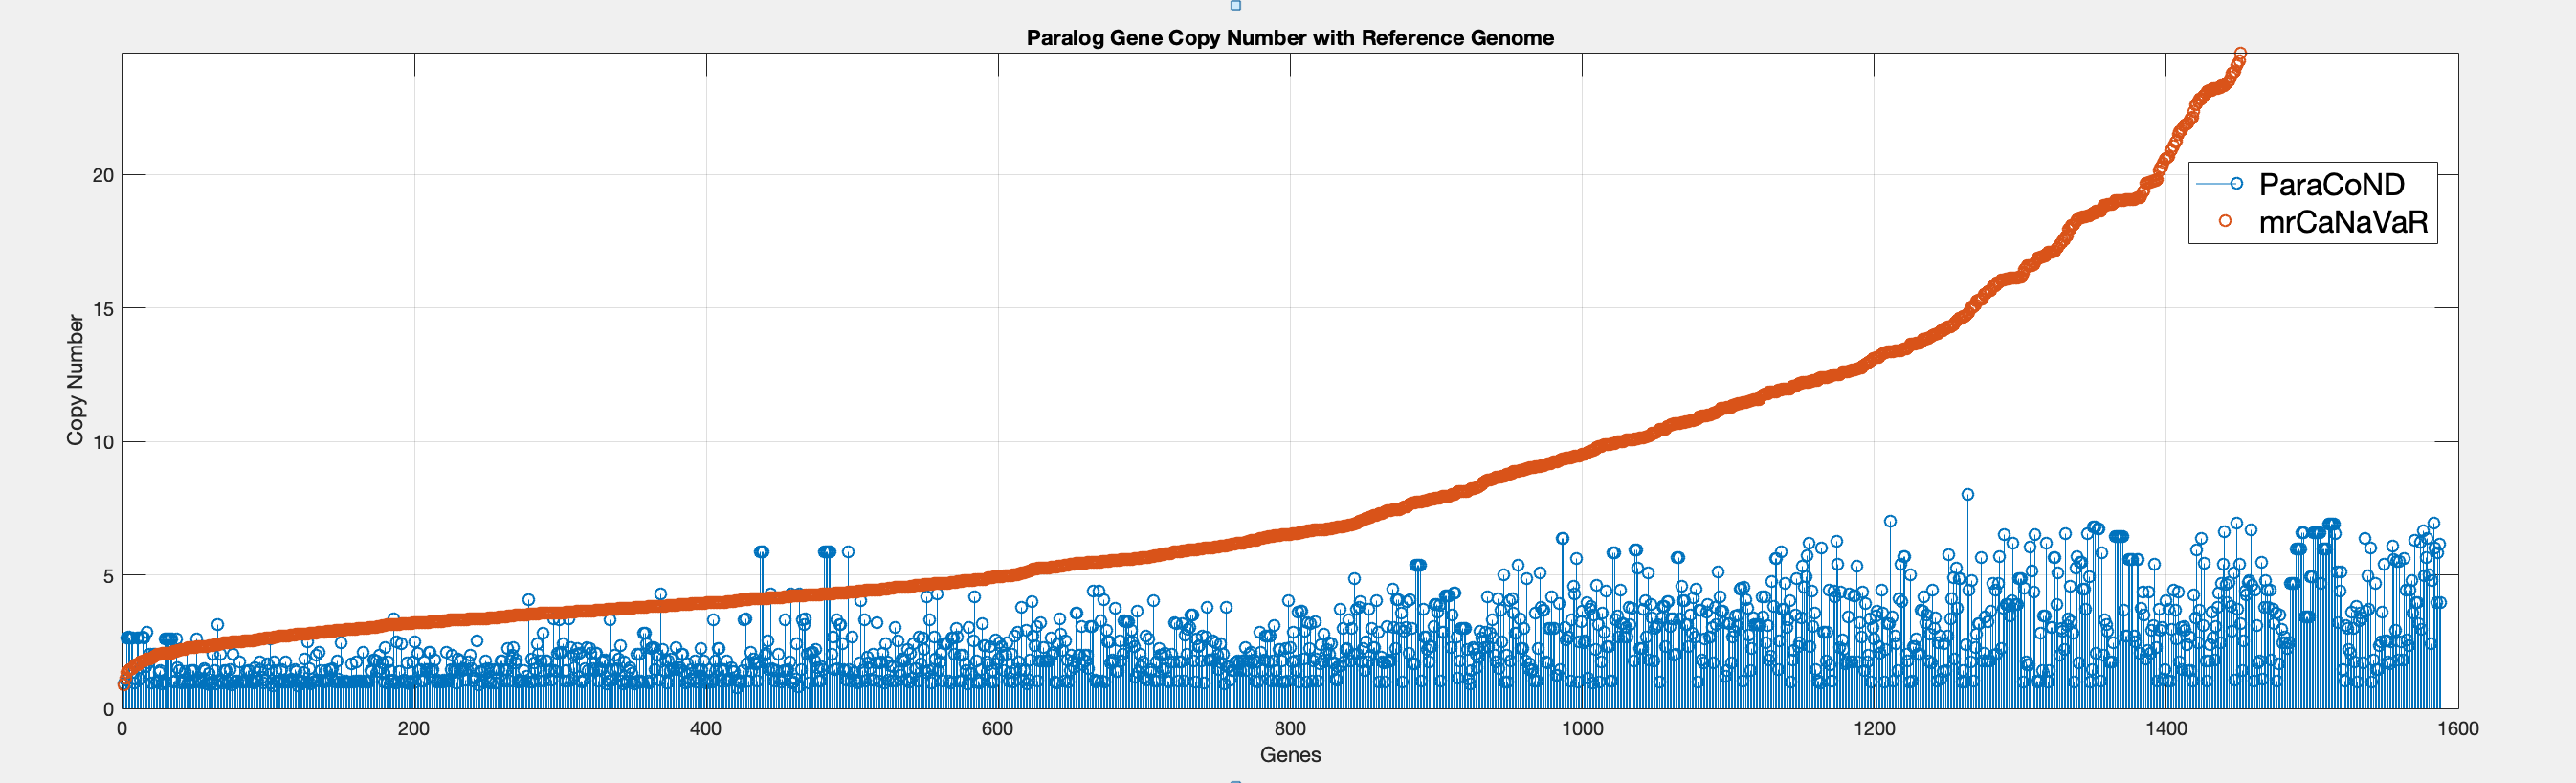
\includegraphics[scale=0.50]{images/reference.png}
    \label{referenceResults}
\end{sidewaysfigure}

Figure \ref{referenceResults} shows the results gathered from both methods using the synthetic data generated from reference genome. Since mrCaNaVaR computes aggregate copy number for paralogs, it can be expected mrCaNaVaR to compute higher than 2. On the other hand, ParaCoND outperforms mrCaNaVaR in this dataset by computing gene copy numbers around 2.

\section{Real Datasets}
We tested ParaCoND with two human genomes: NA12878 from 1000 Genome project and 42S291210 from Turkish Genome project. In general, 30X sequencing coverage is adequate for clinical-level research \cite{shevchenko2016clinical}. Therefore we picked one genome (NA12878) \cite{eberle2017reference} as an example of a human genome sequence with a high coverage (43x) and another genome (42S291210) \cite{alkan2014whole} as an example of relatively low coverage genome (20x).

\section{Results}
In this section, the results of mrCaNaVaR and ParaCoND are compared via several plots. The results include absolute copy numbers of paralog genes (i.e. genes overlapping with segmental duplications). It is not expected the results to match perfectly, however, they should show some level of consistency. We measure the consistency as neighborhood percentages. The neighborhood percentage is the ratio of absolute copy numbers. For example, we say 90\% or more consistent if the following inequality holds; $$\frac{90}{100} \leq \frac{CNV_{ParaCoND}}{CNV_{mrCaNaVaR}} \leq \frac{100}{90} $$.


Table \ref{overlapTable} shows the statistics on the level of consistency between ParaCoND and mrCaNaVaR. 
For NA12878, among 1205 genes for which an absolute copy number is computed by both method, 98 genes show 90\% or more in their neighborhood and for 42S291210, among 1052 genes, 48 genes show 90\% or more in their neighborhood. The reason behind the small difference between two genomes is most likely caused from their sequencing coverage. NA12878 is sequenced 2.15 times more than 42S291210. High sequencing coverage means high quality reads and low sequencing error. 

\begin{table}[!htbp]
    \centering
    \begin{tabular}{lll}
    \hline
    \textbf{Neighborhood Percentage}             & \textbf{NA12878} & \textbf{42S291210}   \\ \hline
    \textbf{\%90 or more} & 103      & 76   \\
    \textbf{\%75 or more} & 250     & 194  \\
    \textbf{\%50 or more} & 561     & 420  \\
    \textbf{\%25 or more} & 923      & 733   \\ \hline
    \textbf{Total}        & 1205    & 1052 \\ \hline
    \end{tabular}
    \caption{Comparison of ParaCoND and mrCaNaVaR. The entries in the table shows the number of genes in each genome with their neighborhood percentages.}
    \label{overlapTable}
\end{table}

Table \ref{overlapVScnvNo} shows how the results are impacted from the value of absolute copy numbers. As the absolute copy numbers grows, their neighborhood percentages decreases. This is mainly because the sensitivity of the methods are getting lower when absolute copy number is high.

\begin{table}[!htbp]
\centering
\caption{Comparison of methods according to copy number values}
\begin{tabular}{lllll}
\hline
\multicolumn{2}{l}{}                                                                         & \textbf{\textless{}10} & \textbf{10-20} & \textbf{20+} \\ \hline
\multicolumn{1}{l|}{\multirow{2}{*}{\textbf{\%90 overlap}}} & \multicolumn{1}{l|}{NA12878}   & 54                        & 27              & 22            \\ \cline{2-5} 
\multicolumn{1}{l|}{}                                       & \multicolumn{1}{l|}{42S291210} & 41                        & 14             & 21            \\ \hline
\multicolumn{1}{l|}{\multirow{2}{*}{\textbf{\%75 overlap}}} & \multicolumn{1}{l|}{NA12878}   & 127                       & 59             & 64           \\ \cline{2-5} 
\multicolumn{1}{l|}{}                                       & \multicolumn{1}{l|}{42S291210} & 105                       & 34             & 55            \\ \hline
\multicolumn{1}{l|}{\multirow{2}{*}{\textbf{\%50 overlap}}} & \multicolumn{1}{l|}{NA12878}   & 280                       & 157             & 124           \\ \cline{2-5} 
\multicolumn{1}{l|}{}                                       & \multicolumn{1}{l|}{42S291210} & 211                       & 105             & 104           \\ \hline
\multicolumn{1}{l|}{\multirow{2}{*}{\textbf{\%25 overlap}}} & \multicolumn{1}{l|}{NA12878}   & 488                       & 243            & 192           \\ \cline{2-5} 
\multicolumn{1}{l|}{}                                       & \multicolumn{1}{l|}{42S291210} & 377                       & 149            & 207           \\ \hline
\end{tabular}
\caption*{The entries in the table indicates the number of genes. First column indicates the genes having absolute copy numbers less than 10, second column indicates the genes having absolute copy numbers between 10 and 20 and the third column indicates the genes having absolute copy numbers more than 20 according to mrCaNaVaR.}
\label{overlapVScnvNo}
\end{table}

We compare the results of two methods via several plots. The first three plots show the results with respect to their neighborhood percentages. We also plot the results according to their absolute copy numbers computed by mrCaNaVaR.

The computed absolute copy numbers for paralog genes by both method can be seen in figure \ref{unfiltered}. In Figure \ref{overlap90}, we filter in the genes that are 90\% or more in the neighborhood. As can be seen in the figure, most of them have an absolute copy number less than 10. Lastly the figure \ref{overlap50} shows the absolute copy numbers computed by both methods in which they overlap 50\% or more.

The comparison of computed absolute copy numbers for genes whose copy number is less than 10 can be seen in figure \ref{lessThan10}. In figure \ref{btw2030}, we compare the absolute copy numbers of genes whose copy numbers vary between 10 and 20. We also compare the absolute copy numbers of genes whose copy number greater than 20 in the figure \ref{greaterThan20}.


\begin{sidewaysfigure}[ht]
    \centering
    \subfloat[NA12878]{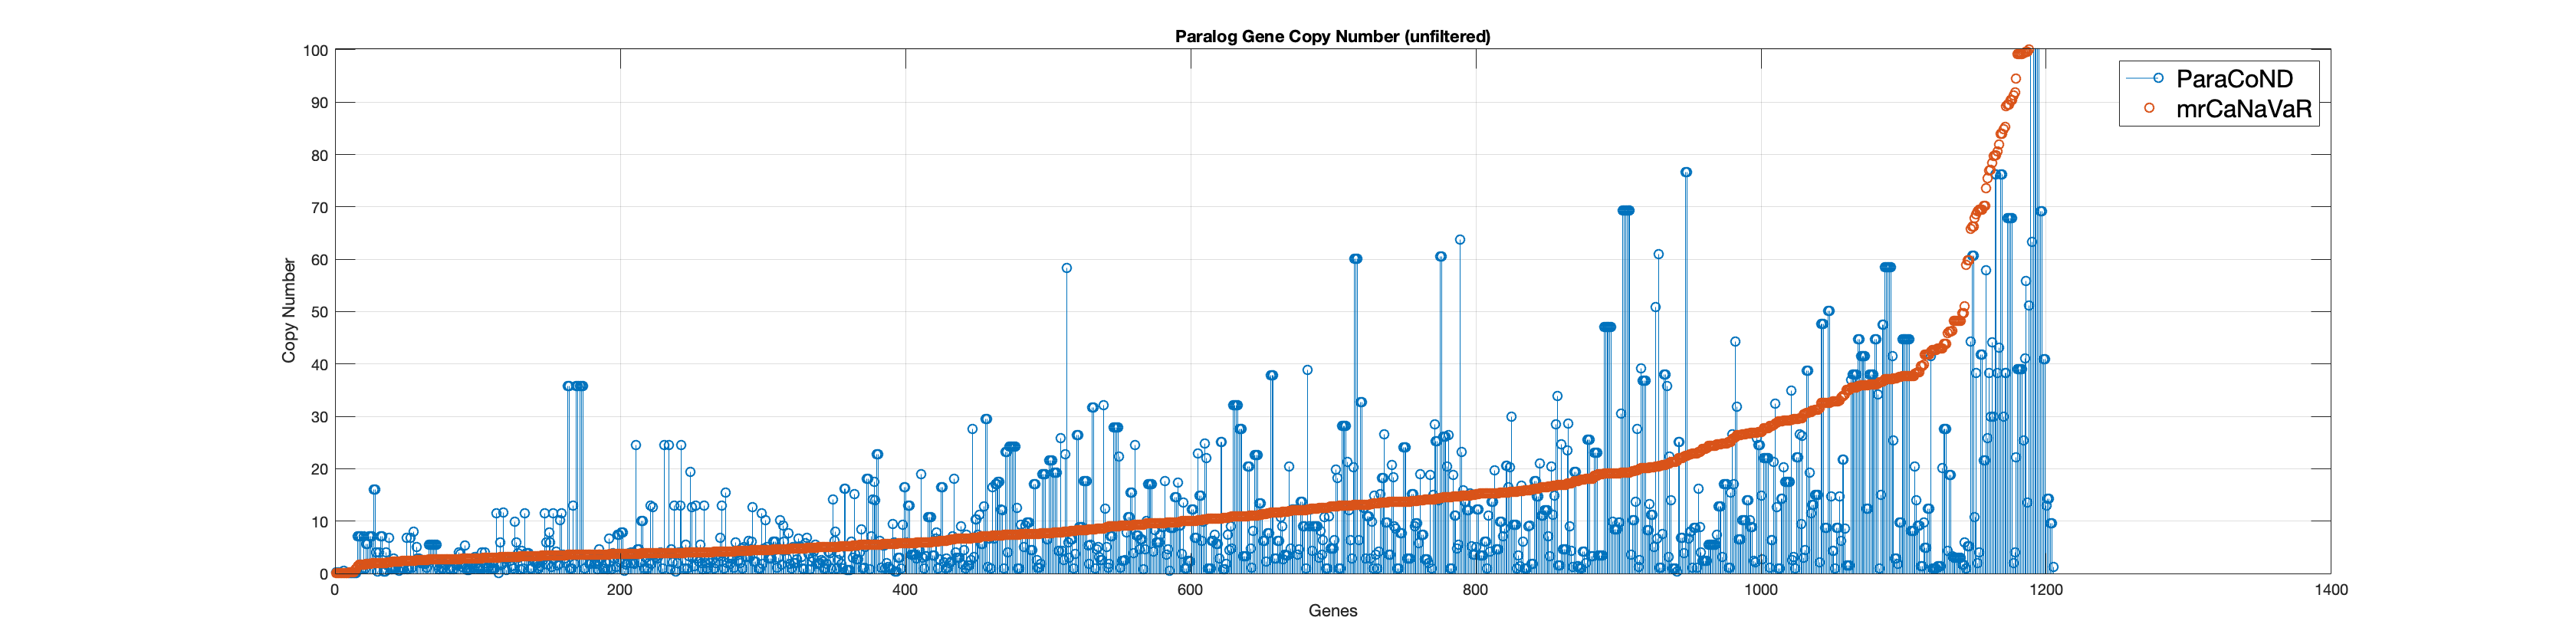
\includegraphics[scale=0.18]{images/na12878/figure1.png}\label{na12878unfiltered}}\quad
    \subfloat[42S291210]{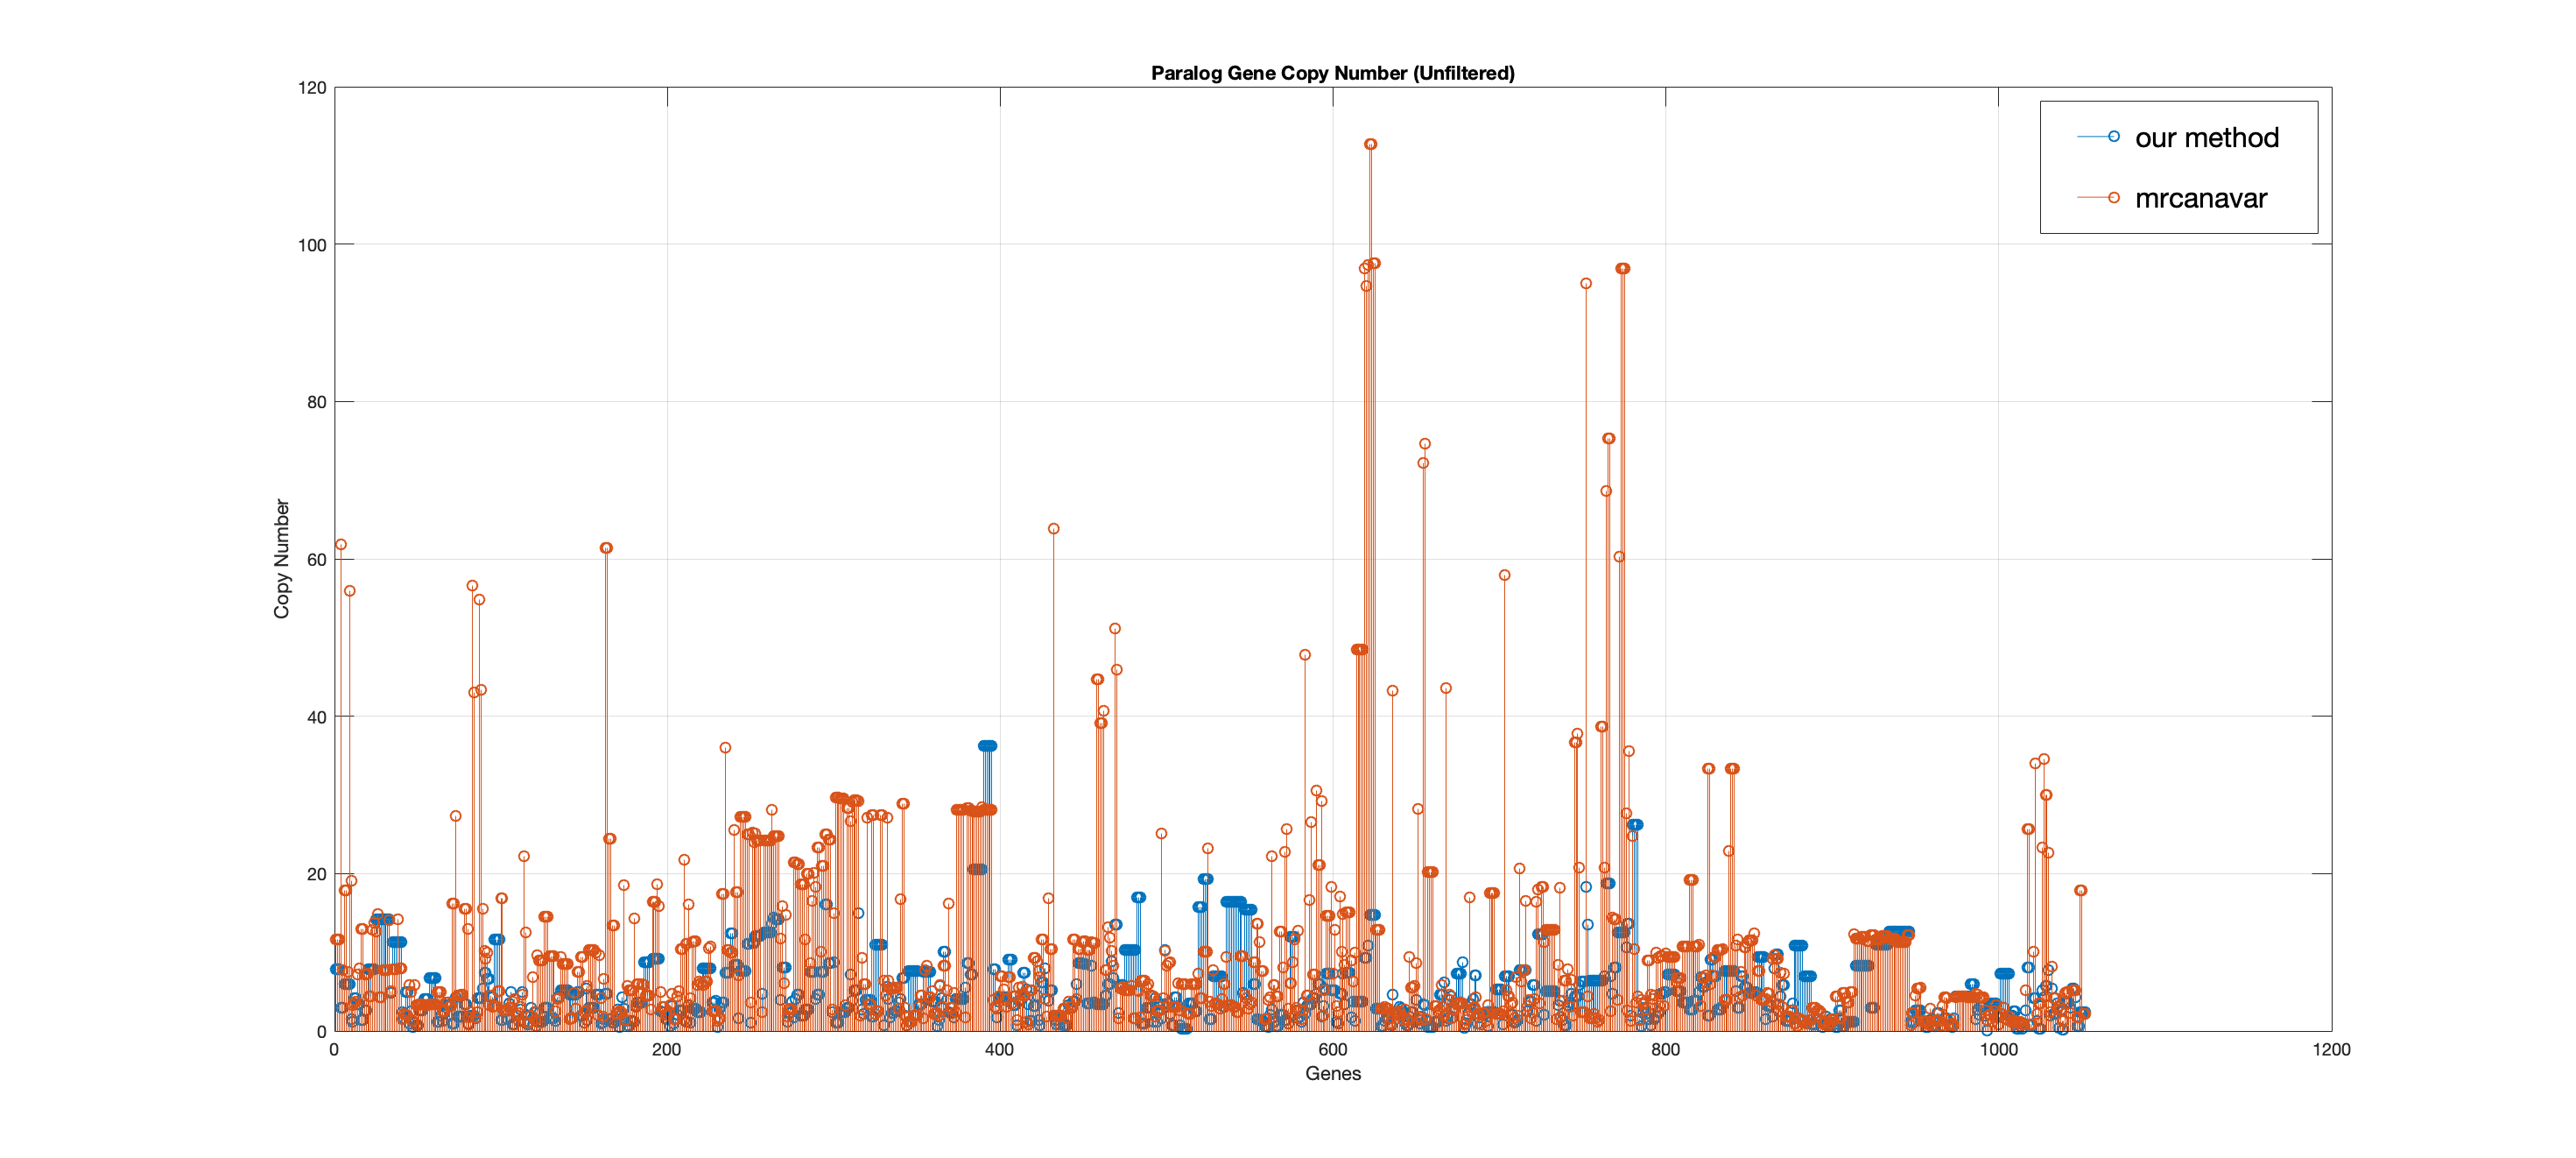
\includegraphics[scale=0.20]{images/42/figure1.png}\label{42unfiltered}}
    \caption{Absolute copy numbers of genes overlapping with segmental duplications}
    \label{unfiltered}
\end{sidewaysfigure}

\begin{figure}
    \centering
    \subfloat[NA12878]{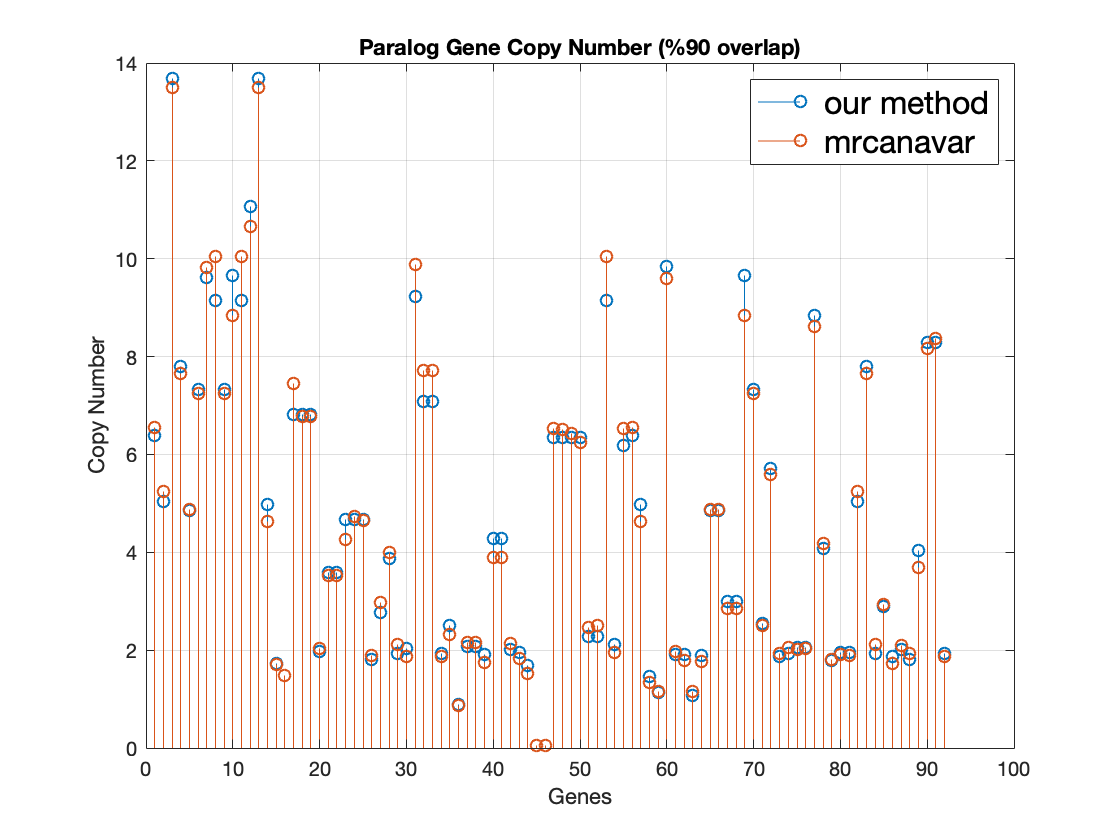
\includegraphics[scale=0.30]{images/na12878/figure2.png}\label{na12878overlap90}}\quad
    \subfloat[42S291210]{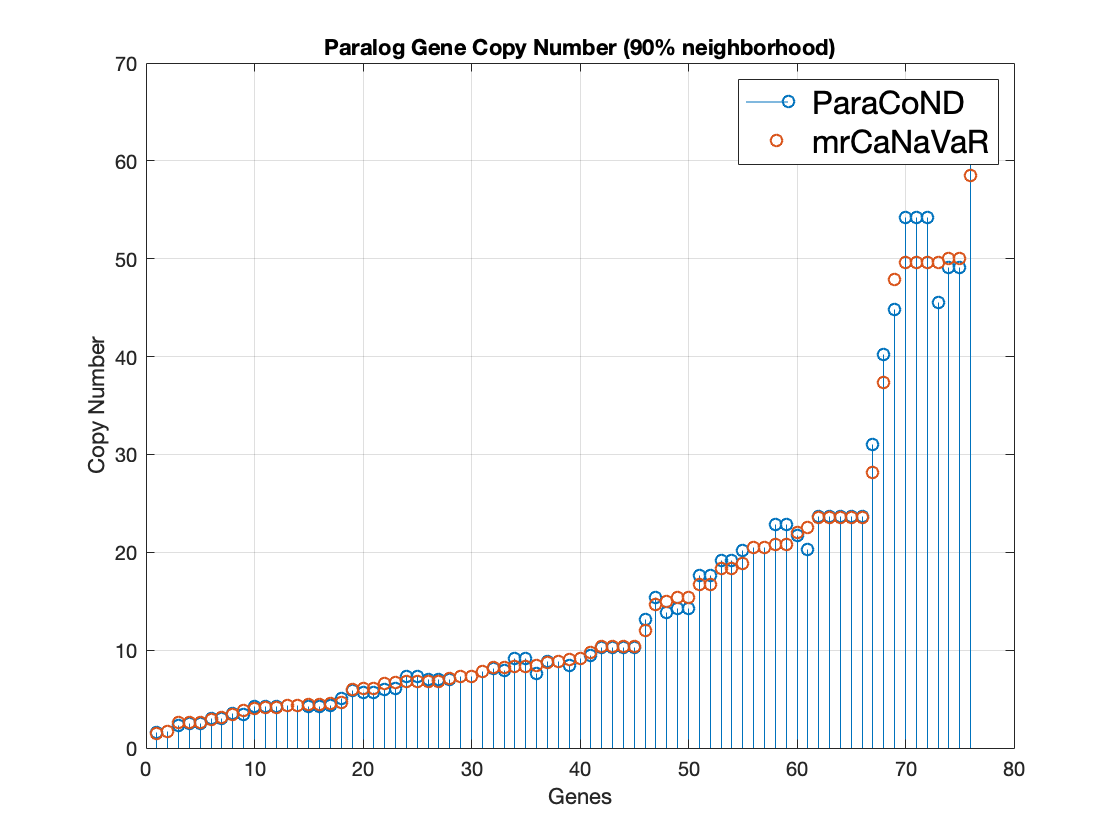
\includegraphics[scale=0.30]{images/42/figure2.png}\label{42overlap90}}
    \caption{Absolute copy numbers of genes showing \%90 overlapping by both methods}
    \label{overlap90}
\end{figure}

\begin{sidewaysfigure}[ht]
    \centering
    \subfloat[NA12878]{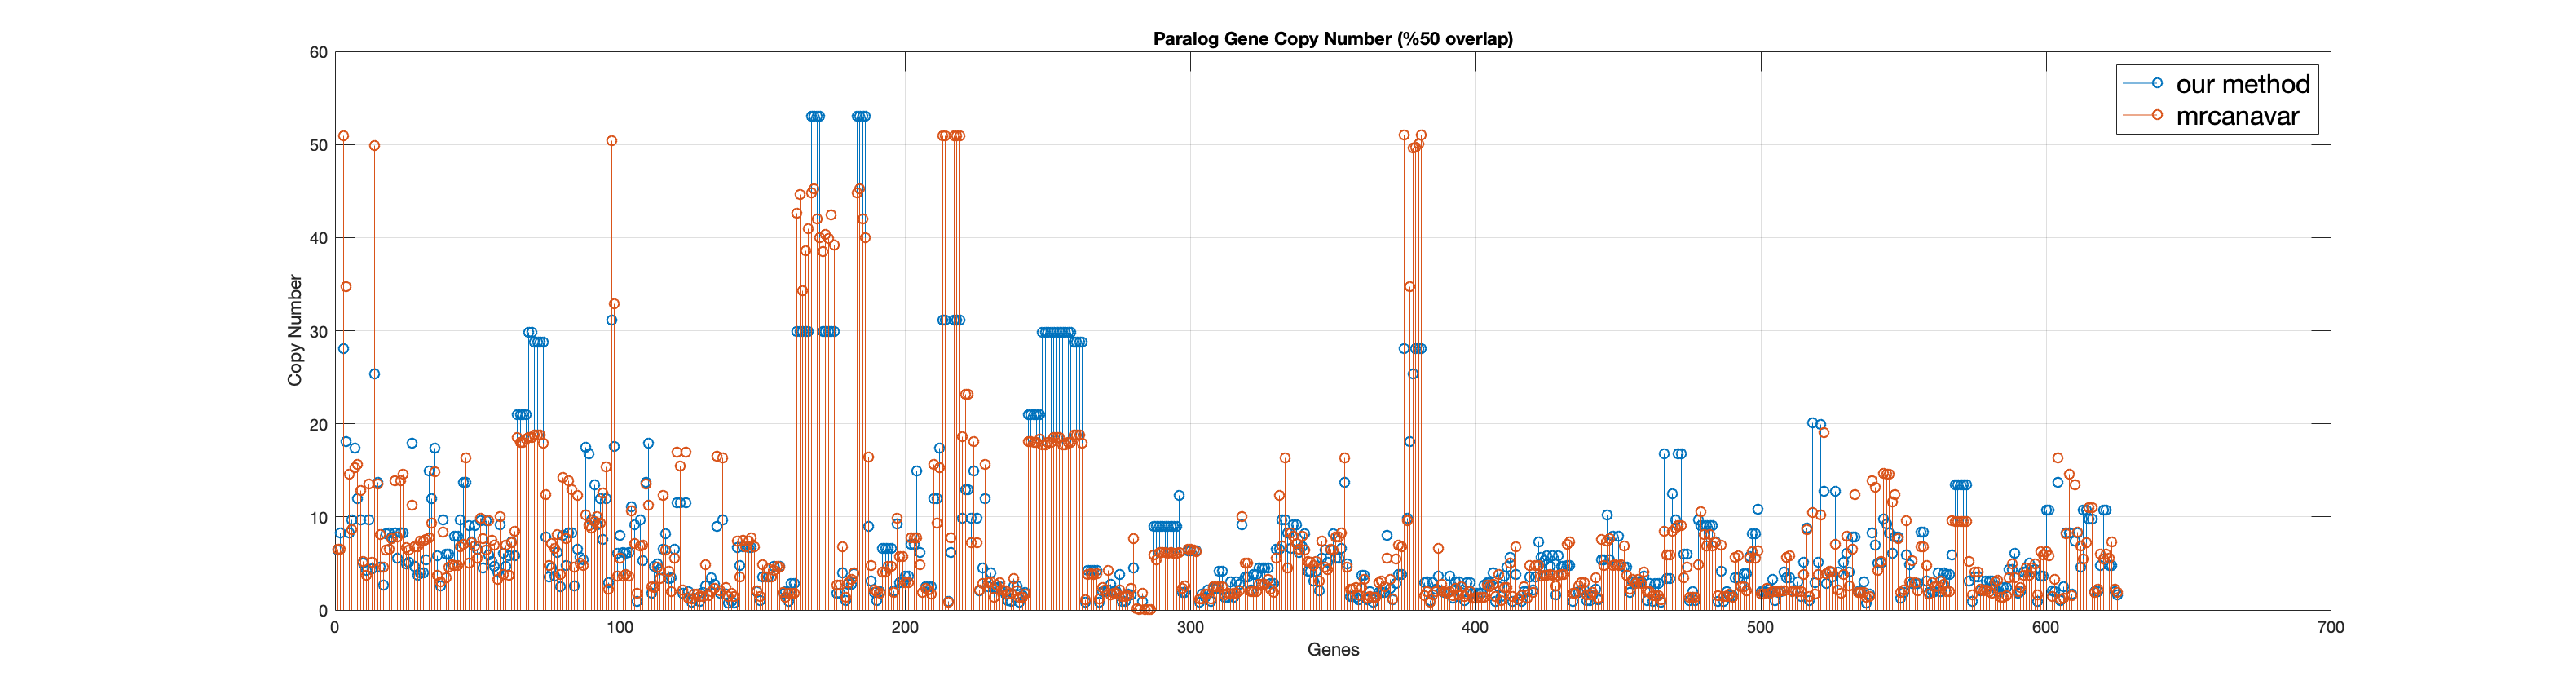
\includegraphics[scale=0.18]{images/na12878/figure3.png}\label{na12878overlap50}}\quad
    \subfloat[42S291210]{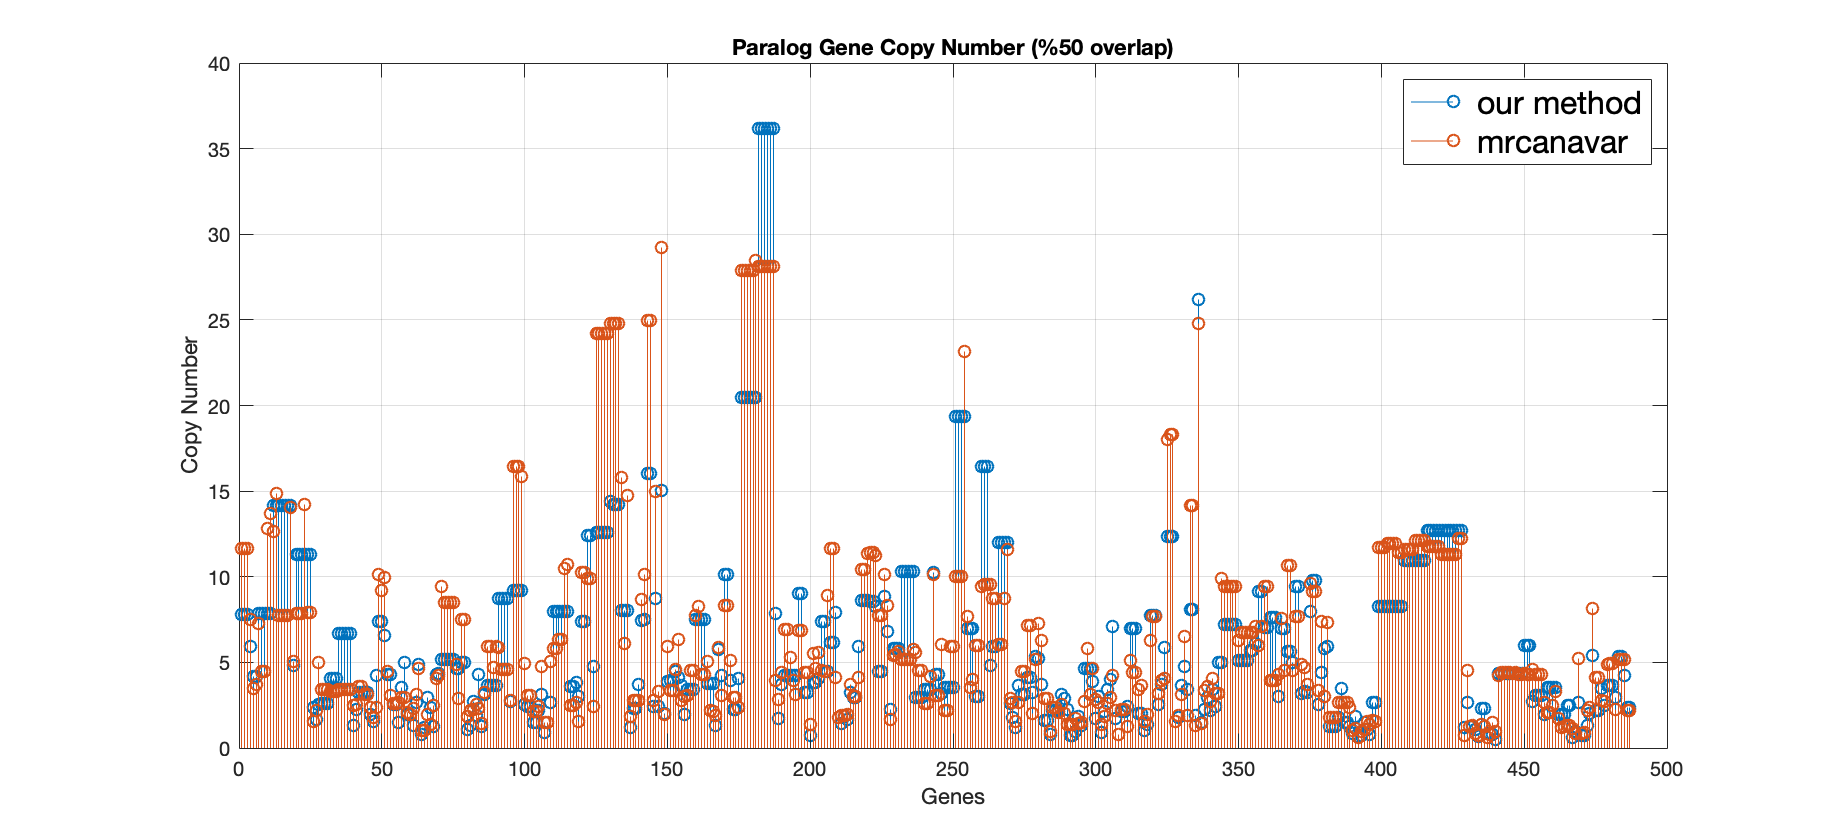
\includegraphics[scale=0.30]{images/42/figure3.png}\label{42overlap50}}
    \caption{Absolute copy numbers of genes showing \%50 overlapping by both methods}
    \label{overlap50}
\end{sidewaysfigure}


\begin{sidewaysfigure}[ht]
    \centering
    \subfloat[NA12878]{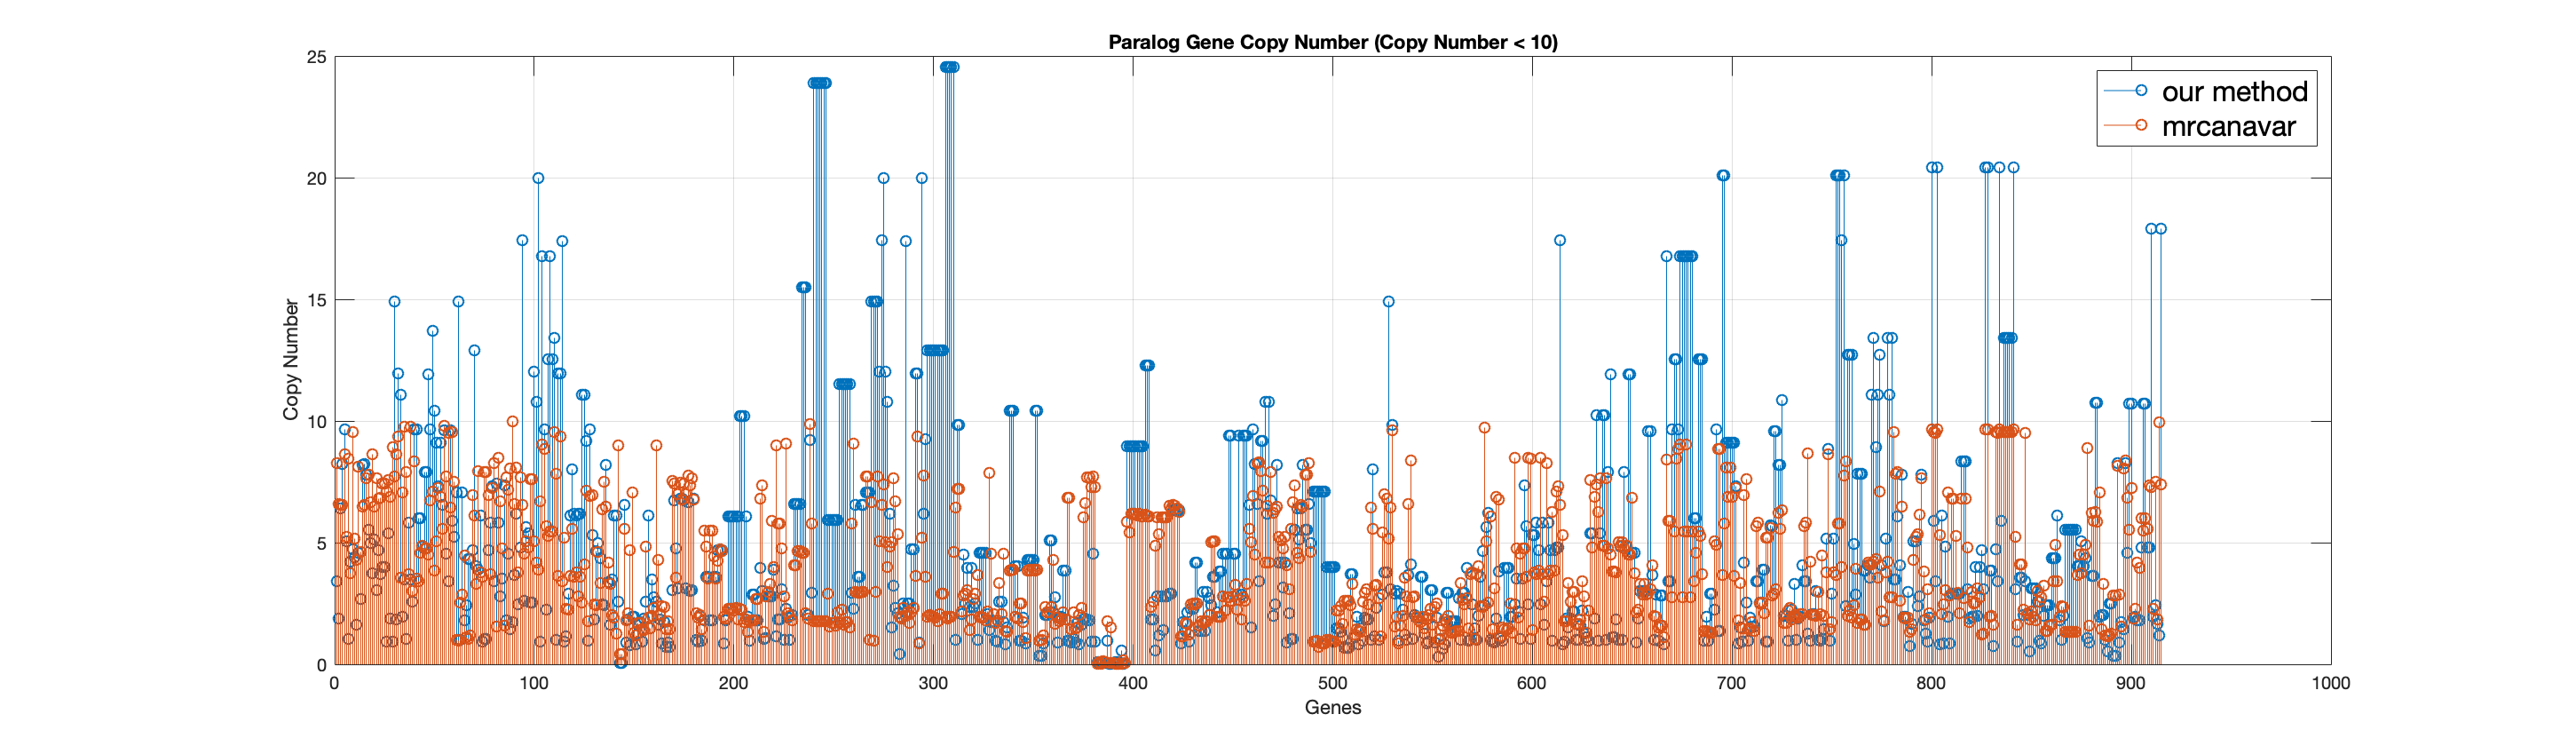
\includegraphics[scale=0.20]{images/na12878/figure4.png}\label{na12878lt10}}\quad
    \subfloat[42S291210]{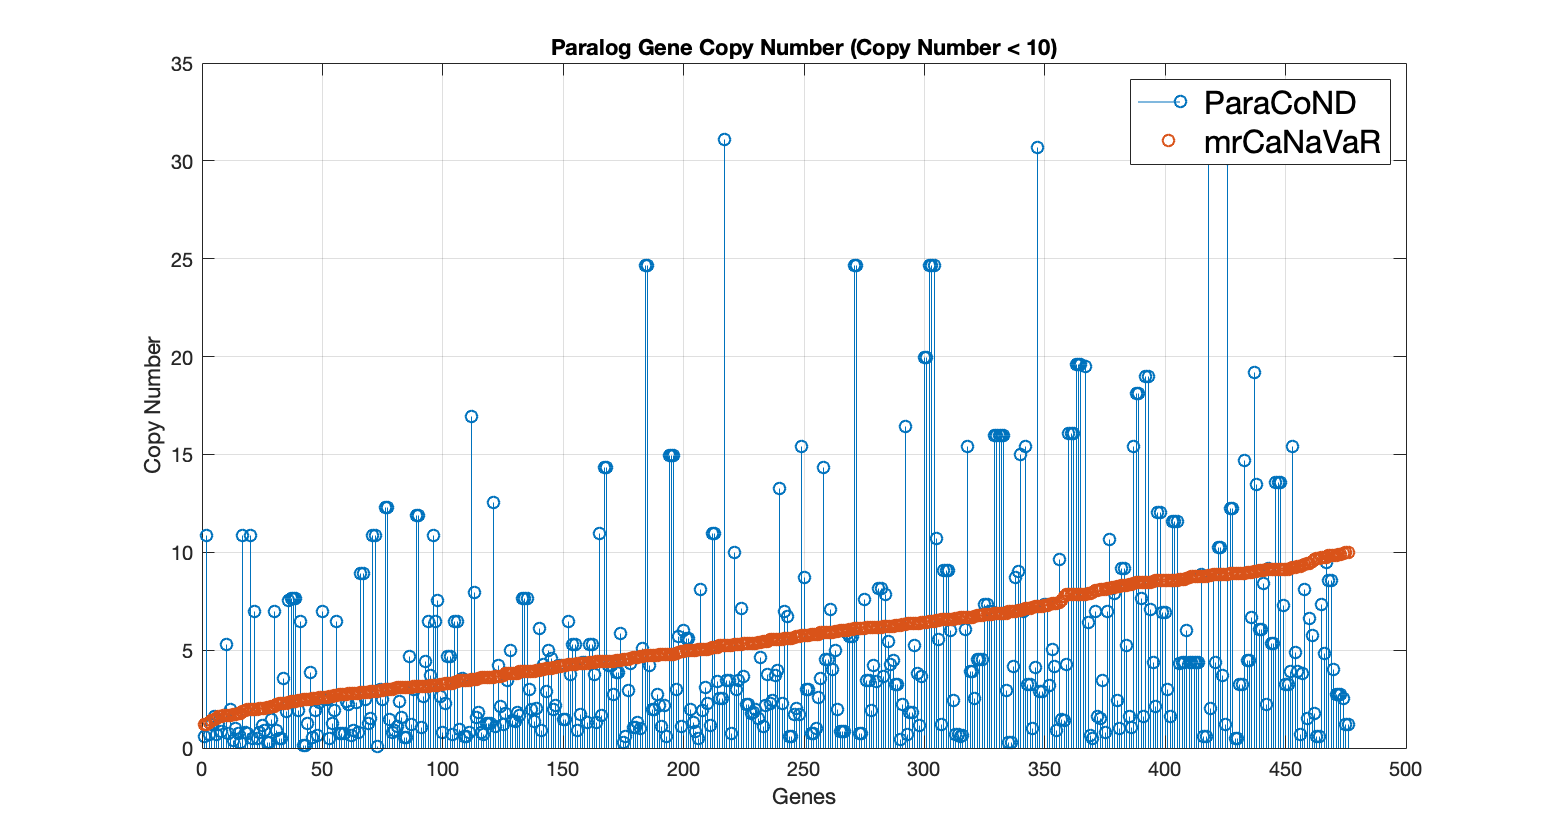
\includegraphics[scale=0.20]{images/42/figure4.png}\label{42lt10}}
    \caption{Absolute copy numbers of genes whose copy numbers are less than 10 according to mrCaNaVaR}
    \label{lessThan10}
\end{sidewaysfigure}

\begin{figure}
    \centering
    \subfloat[NA12878]{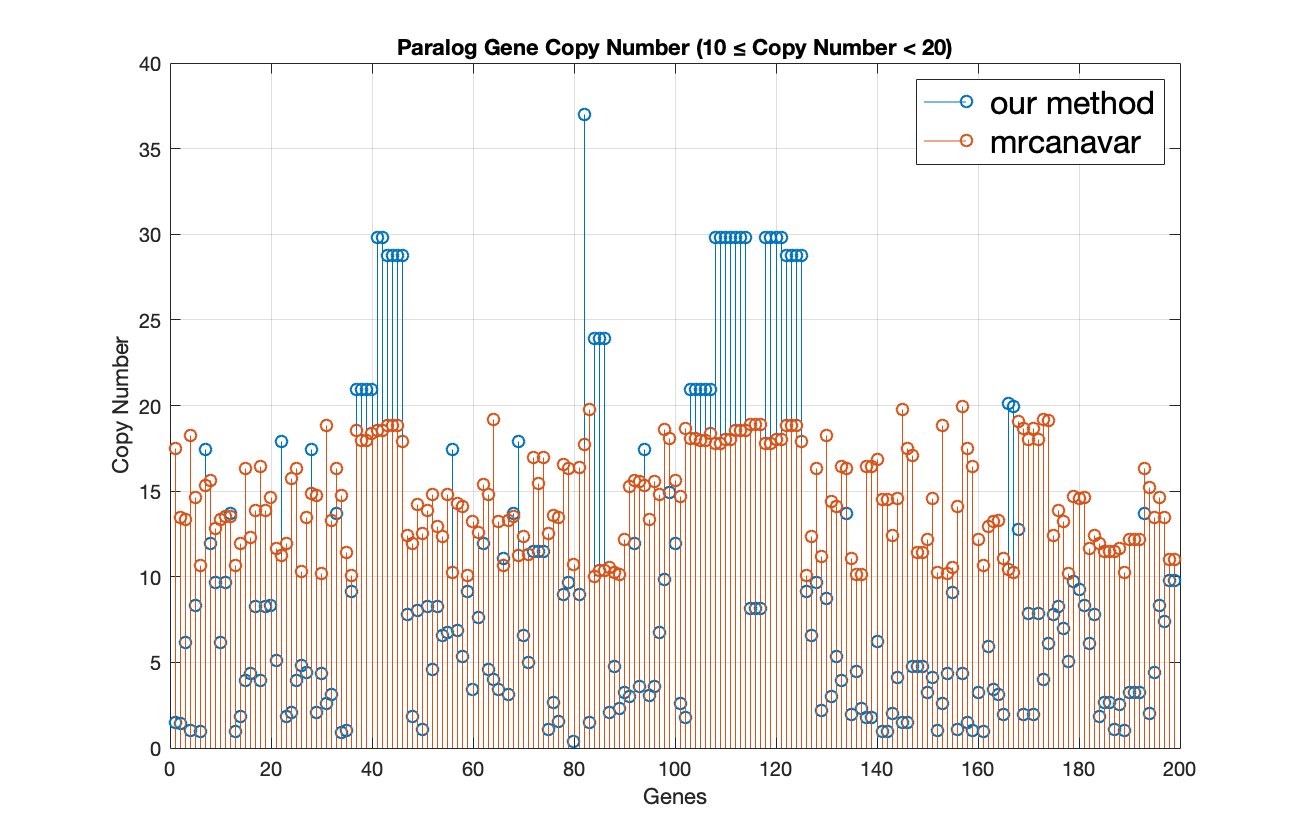
\includegraphics[scale=0.30]{images/na12878/figure5.png}\label{na12878btw1020}}\quad
    \subfloat[42S291210]{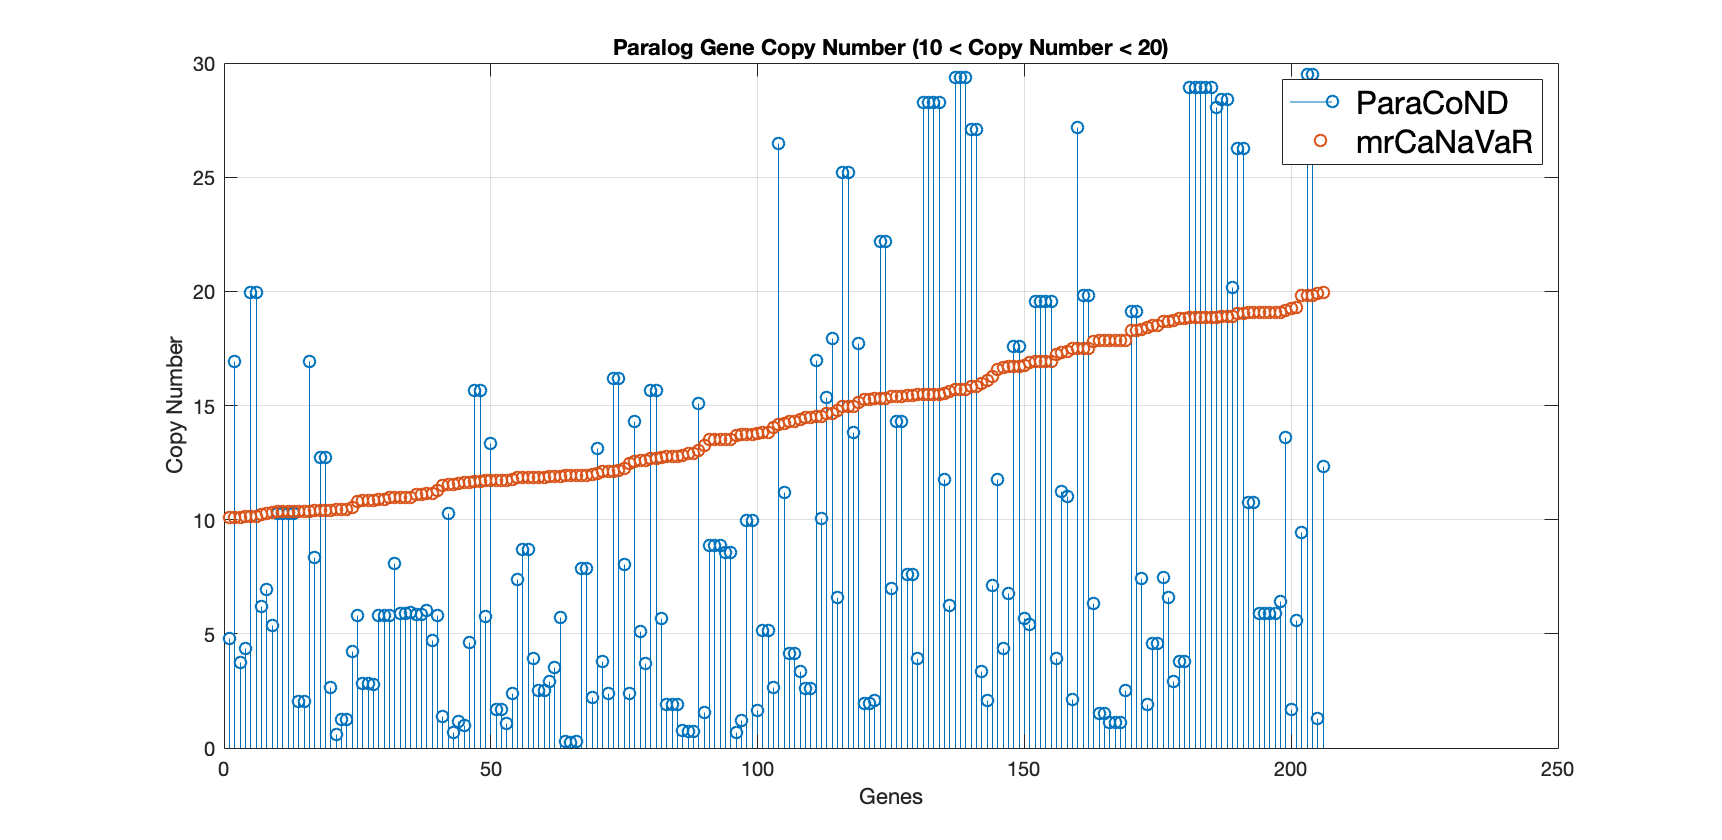
\includegraphics[scale=0.25]{images/42/figure5.png}\label{42btw1020}}
    \caption{Absolute copy numbers of genes whose copy numbers are between 10 and 20 according to mrCaNaVaR}
    \label{btw2030}
\end{figure}


\begin{figure}
    \centering
    \subfloat[NA12878]{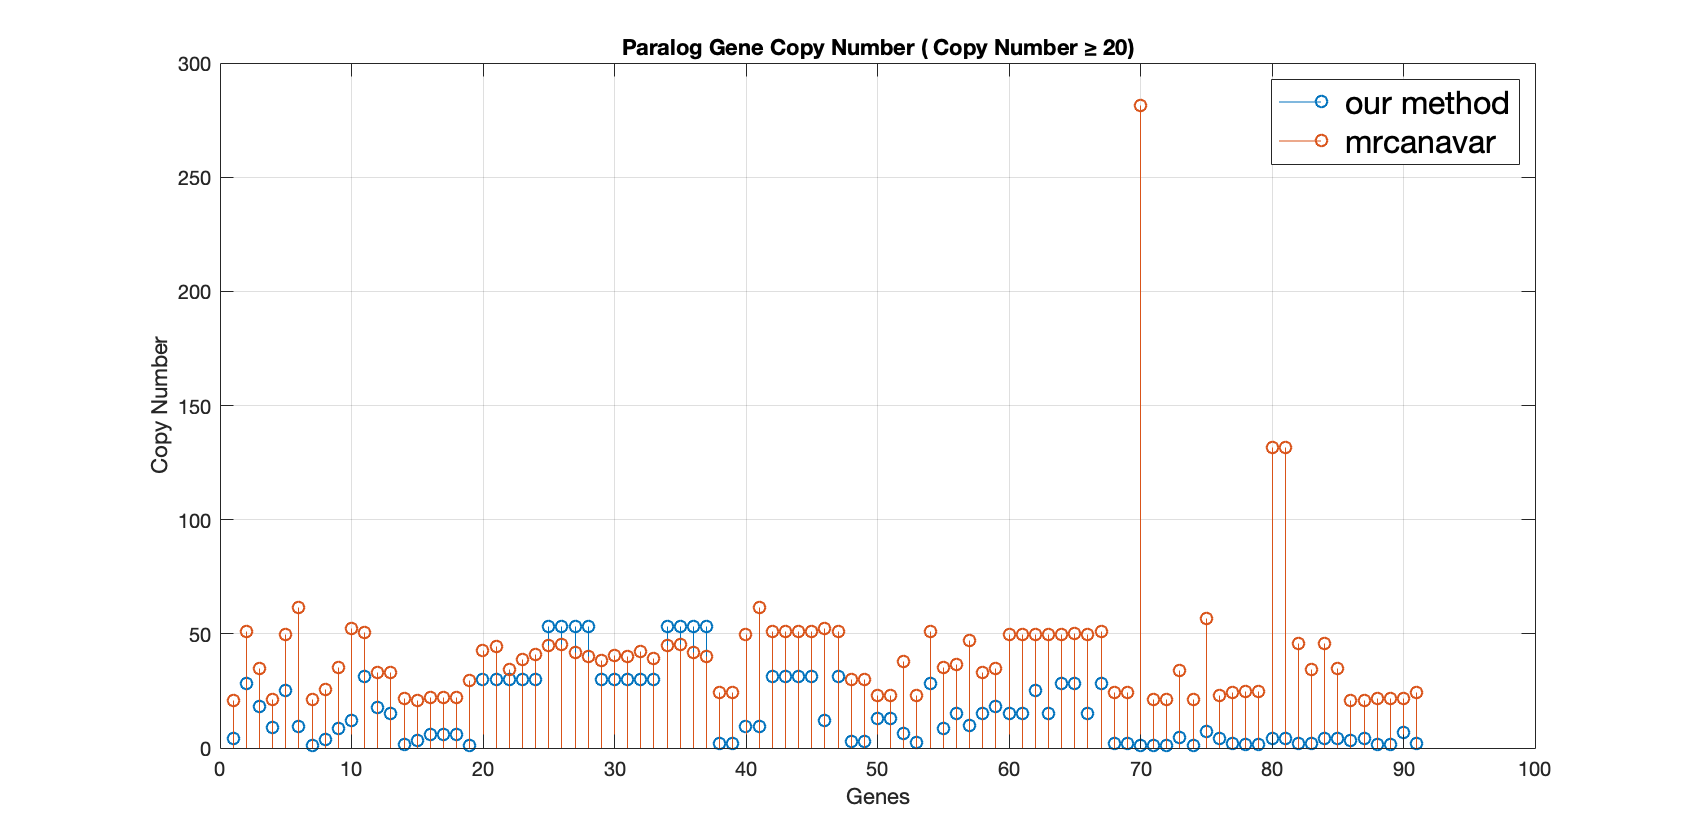
\includegraphics[scale=0.25]{images/na12878/figure6.png}\label{na12878gt20}}\quad
    \subfloat[42S291210]{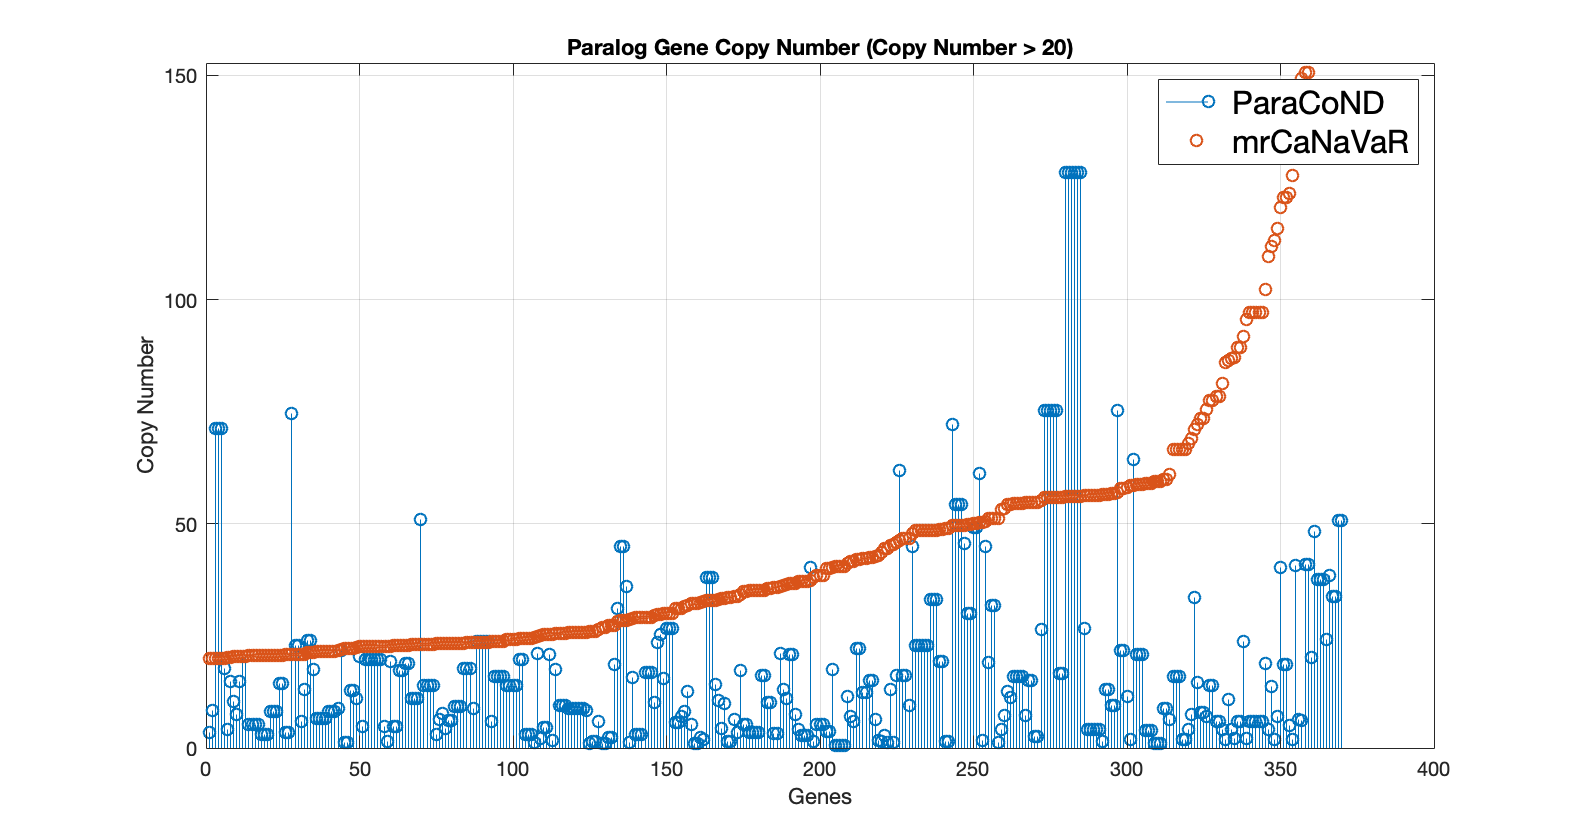
\includegraphics[scale=0.20]{images/42/figure6.png}\label{42gt20}}
    \caption{Absolute copy numbers of genes whose copy numbers are greater than 20 according to mrCaNaVaR}
    \label{greaterThan20}
\end{figure}